\documentclass[tikz,border=1mm]{standalone}
% Shared publication styles; labels designed for 170 mm inclusion width.
\usepackage[T1]{fontenc}
\usepackage{lmodern}
\usepackage{amsmath}
\usepackage{tikz}
\usepackage{pgfplots}
\pgfplotsset{compat=1.18}
\usetikzlibrary{arrows.meta,positioning,calc,fit,backgrounds,shapes.geometric,patterns,decorations.pathreplacing,circuits.logic.US}
\definecolor{ink}{HTML}{263238}
\definecolor{muted}{HTML}{60717D}
\definecolor{grid}{HTML}{DCE5EA}
\definecolor{normal}{HTML}{4C78A8}
\definecolor{compact}{HTML}{59A14F}
\definecolor{june}{HTML}{8A6BBE}
\definecolor{warn}{HTML}{C18523}
\definecolor{bad}{HTML}{BC514C}
\definecolor{phasezero}{HTML}{DBEAF8}
\definecolor{phaseone}{HTML}{DFEFD9}
\definecolor{phasetwo}{HTML}{FFF1C8}
\definecolor{phasethree}{HTML}{ECE1F6}
\tikzset{
  every picture/.style={font=\sffamily\fontsize{8}{9.5}\selectfont,text=ink},
  >=Latex,
  box/.style={draw=ink!60,fill=white,rounded corners=1.2pt,align=center,inner sep=4pt,line width=.55pt},
  flow/.style={-{Latex[length=1.7mm,width=1.2mm]},draw=ink,line width=.65pt},
  control/.style={flow,dashed,draw=muted},
  retry/.style={flow,draw=warn},
  paneltitle/.style={font=\sffamily\bfseries\fontsize{9}{10.5}\selectfont,anchor=west},
  smallnote/.style={font=\sffamily\fontsize{7}{8.5}\selectfont,text=muted,align=left},
  gridline/.style={draw=grid,line width=.2pt},
}
\pgfplotsset{every axis/.append style={
  font=\sffamily\fontsize{8}{9.5}\selectfont,
  label style={font=\sffamily\fontsize{8}{9.5}\selectfont},
  tick label style={font=\sffamily\fontsize{7.5}{9}\selectfont},
  legend style={font=\sffamily\fontsize{7.5}{9}\selectfont,draw=none,fill=none},
  axis line style={draw=ink!65},tick style={draw=ink!65},
  grid style={draw=grid},
}}

\begin{document}
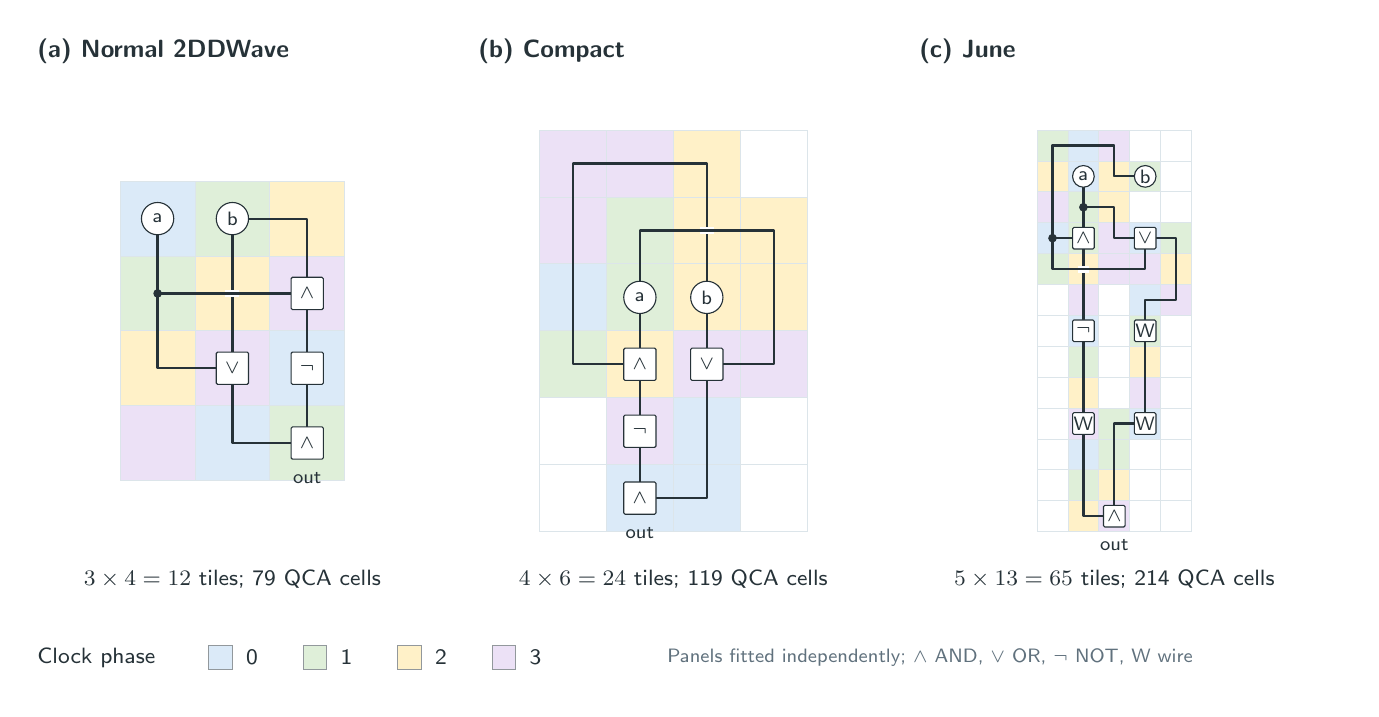
\begin{tikzpicture}[x=1mm,y=-1mm]
\path[use as bounding box] (0,0) rectangle (168,84);
\node[paneltitle] at (0,3) {(a) Normal 2DDWave};
\draw[fill=phasezero,draw=grid,line width=.3pt] (11.750,19.500) rectangle (21.250,29.000);
\draw[fill=phaseone,draw=grid,line width=.3pt] (21.250,19.500) rectangle (30.750,29.000);
\draw[fill=phasetwo,draw=grid,line width=.3pt] (30.750,19.500) rectangle (40.250,29.000);
\draw[fill=phaseone,draw=grid,line width=.3pt] (11.750,29.000) rectangle (21.250,38.500);
\draw[fill=phasetwo,draw=grid,line width=.3pt] (21.250,29.000) rectangle (30.750,38.500);
\draw[fill=phasethree,draw=grid,line width=.3pt] (30.750,29.000) rectangle (40.250,38.500);
\draw[fill=phasetwo,draw=grid,line width=.3pt] (11.750,38.500) rectangle (21.250,48.000);
\draw[fill=phasethree,draw=grid,line width=.3pt] (21.250,38.500) rectangle (30.750,48.000);
\draw[fill=phasezero,draw=grid,line width=.3pt] (30.750,38.500) rectangle (40.250,48.000);
\draw[fill=phasethree,draw=grid,line width=.3pt] (11.750,48.000) rectangle (21.250,57.500);
\draw[fill=phasezero,draw=grid,line width=.3pt] (21.250,48.000) rectangle (30.750,57.500);
\draw[fill=phaseone,draw=grid,line width=.3pt] (30.750,48.000) rectangle (40.250,57.500);
\draw[ink,line width=.8pt,line join=round] (35.500,43.250) -- (35.500,52.750);
\draw[ink,line width=.8pt,line join=round] (35.500,33.750) -- (35.500,43.250);
\draw[ink,line width=.8pt,line join=round] (16.500,24.250) -- (16.500,33.750) -- (16.500,43.250) -- (26.000,43.250);
\draw[ink,line width=.8pt,line join=round] (26.000,24.250) -- (35.500,24.250) -- (35.500,33.750);
\draw[ink,line width=.8pt,line join=round] (26.000,43.250) -- (26.000,52.750) -- (35.500,52.750);
\draw[ink,line width=.8pt,line join=round] (26.000,24.250) -- (26.000,33.750) -- (26.000,43.250);
\draw[ink,line width=.8pt,line join=round] (16.500,24.250) -- (16.500,33.750) -- (26.000,33.750) -- (35.500,33.750);
\draw[white,line width=2.5pt] (25.100,33.750) -- (26.900,33.750);
\draw[ink,line width=.8pt] (25.100,33.750) -- (26.900,33.750);
\fill[ink] (16.500,33.750) circle (.55mm);
\node[circle,draw=ink,fill=white,minimum size=4.10mm,inner sep=0pt,font=\sffamily\fontsize{7}{8}\selectfont] (l0n0) at (16.500,24.250) {a};
\node[circle,draw=ink,fill=white,minimum size=4.10mm,inner sep=0pt,font=\sffamily\fontsize{7}{8}\selectfont] (l0n1) at (26.000,24.250) {b};
\node[rectangle,rounded corners=.5pt,draw=ink,fill=white,minimum size=4.10mm,inner sep=0pt,font=\sffamily\fontsize{7}{8}\selectfont] (l0n2) at (35.500,52.750) {$\wedge$};
\node[anchor=north,font=\sffamily\fontsize{7}{8}\selectfont] at (35.500,55.200) {out};
\node[rectangle,rounded corners=.5pt,draw=ink,fill=white,minimum size=4.10mm,inner sep=0pt,font=\sffamily\fontsize{7}{8}\selectfont] (l0n3) at (26.000,43.250) {$\vee$};
\node[rectangle,rounded corners=.5pt,draw=ink,fill=white,minimum size=4.10mm,inner sep=0pt,font=\sffamily\fontsize{7}{8}\selectfont] (l0n4) at (35.500,33.750) {$\wedge$};
\node[rectangle,rounded corners=.5pt,draw=ink,fill=white,minimum size=4.10mm,inner sep=0pt,font=\sffamily\fontsize{7}{8}\selectfont] (l0n5) at (35.500,43.250) {$\neg$};
\node[align=center] at (26,70) {$3\times4=12$ tiles; 79 QCA cells};
\node[paneltitle] at (56,3) {(b) Compact};
\draw[fill=phasethree,draw=grid,line width=.3pt] (65.000,13.000) rectangle (73.500,21.500);
\draw[fill=phasethree,draw=grid,line width=.3pt] (73.500,13.000) rectangle (82.000,21.500);
\draw[fill=phasetwo,draw=grid,line width=.3pt] (82.000,13.000) rectangle (90.500,21.500);
\draw[fill=white,draw=grid,line width=.3pt] (90.500,13.000) rectangle (99.000,21.500);
\draw[fill=phasethree,draw=grid,line width=.3pt] (65.000,21.500) rectangle (73.500,30.000);
\draw[fill=phaseone,draw=grid,line width=.3pt] (73.500,21.500) rectangle (82.000,30.000);
\draw[fill=phasetwo,draw=grid,line width=.3pt] (82.000,21.500) rectangle (90.500,30.000);
\draw[fill=phasetwo,draw=grid,line width=.3pt] (90.500,21.500) rectangle (99.000,30.000);
\draw[fill=phasezero,draw=grid,line width=.3pt] (65.000,30.000) rectangle (73.500,38.500);
\draw[fill=phaseone,draw=grid,line width=.3pt] (73.500,30.000) rectangle (82.000,38.500);
\draw[fill=phasetwo,draw=grid,line width=.3pt] (82.000,30.000) rectangle (90.500,38.500);
\draw[fill=phasetwo,draw=grid,line width=.3pt] (90.500,30.000) rectangle (99.000,38.500);
\draw[fill=phaseone,draw=grid,line width=.3pt] (65.000,38.500) rectangle (73.500,47.000);
\draw[fill=phasetwo,draw=grid,line width=.3pt] (73.500,38.500) rectangle (82.000,47.000);
\draw[fill=phasethree,draw=grid,line width=.3pt] (82.000,38.500) rectangle (90.500,47.000);
\draw[fill=phasethree,draw=grid,line width=.3pt] (90.500,38.500) rectangle (99.000,47.000);
\draw[fill=white,draw=grid,line width=.3pt] (65.000,47.000) rectangle (73.500,55.500);
\draw[fill=phasethree,draw=grid,line width=.3pt] (73.500,47.000) rectangle (82.000,55.500);
\draw[fill=phasezero,draw=grid,line width=.3pt] (82.000,47.000) rectangle (90.500,55.500);
\draw[fill=white,draw=grid,line width=.3pt] (90.500,47.000) rectangle (99.000,55.500);
\draw[fill=white,draw=grid,line width=.3pt] (65.000,55.500) rectangle (73.500,64.000);
\draw[fill=phasezero,draw=grid,line width=.3pt] (73.500,55.500) rectangle (82.000,64.000);
\draw[fill=phasezero,draw=grid,line width=.3pt] (82.000,55.500) rectangle (90.500,64.000);
\draw[fill=white,draw=grid,line width=.3pt] (90.500,55.500) rectangle (99.000,64.000);
\draw[ink,line width=.8pt,line join=round] (77.750,34.250) -- (77.750,42.750);
\draw[ink,line width=.8pt,line join=round] (77.750,34.250) -- (77.750,25.750) -- (86.250,25.750) -- (94.750,25.750) -- (94.750,34.250) -- (94.750,42.750) -- (86.250,42.750);
\draw[ink,line width=.8pt,line join=round] (86.250,34.250) -- (86.250,25.750) -- (86.250,17.250) -- (77.750,17.250) -- (69.250,17.250) -- (69.250,25.750) -- (69.250,34.250) -- (69.250,42.750) -- (77.750,42.750);
\draw[ink,line width=.8pt,line join=round] (86.250,34.250) -- (86.250,42.750);
\draw[ink,line width=.8pt,line join=round] (77.750,42.750) -- (77.750,51.250);
\draw[ink,line width=.8pt,line join=round] (86.250,42.750) -- (86.250,51.250) -- (86.250,59.750) -- (77.750,59.750);
\draw[ink,line width=.8pt,line join=round] (77.750,51.250) -- (77.750,59.750);
\draw[white,line width=2.5pt] (85.350,25.750) -- (87.150,25.750);
\draw[ink,line width=.8pt] (85.350,25.750) -- (87.150,25.750);
\node[circle,draw=ink,fill=white,minimum size=4.10mm,inner sep=0pt,font=\sffamily\fontsize{7}{8}\selectfont] (l1n0) at (77.750,34.250) {a};
\node[circle,draw=ink,fill=white,minimum size=4.10mm,inner sep=0pt,font=\sffamily\fontsize{7}{8}\selectfont] (l1n1) at (86.250,34.250) {b};
\node[rectangle,rounded corners=.5pt,draw=ink,fill=white,minimum size=4.10mm,inner sep=0pt,font=\sffamily\fontsize{7}{8}\selectfont] (l1n2) at (77.750,59.750) {$\wedge$};
\node[anchor=north,font=\sffamily\fontsize{7}{8}\selectfont] at (77.750,62.200) {out};
\node[rectangle,rounded corners=.5pt,draw=ink,fill=white,minimum size=4.10mm,inner sep=0pt,font=\sffamily\fontsize{7}{8}\selectfont] (l1n3) at (77.750,42.750) {$\wedge$};
\node[rectangle,rounded corners=.5pt,draw=ink,fill=white,minimum size=4.10mm,inner sep=0pt,font=\sffamily\fontsize{7}{8}\selectfont] (l1n4) at (86.250,42.750) {$\vee$};
\node[rectangle,rounded corners=.5pt,draw=ink,fill=white,minimum size=4.10mm,inner sep=0pt,font=\sffamily\fontsize{7}{8}\selectfont] (l1n5) at (77.750,51.250) {$\neg$};
\node[align=center] at (82,70) {$4\times6=24$ tiles; 119 QCA cells};
\node[paneltitle] at (112,3) {(c) June};
\draw[fill=phaseone,draw=grid,line width=.3pt] (128.192,13.000) rectangle (132.115,16.923);
\draw[fill=phasezero,draw=grid,line width=.3pt] (132.115,13.000) rectangle (136.038,16.923);
\draw[fill=phasethree,draw=grid,line width=.3pt] (136.038,13.000) rectangle (139.962,16.923);
\draw[fill=white,draw=grid,line width=.3pt] (139.962,13.000) rectangle (143.885,16.923);
\draw[fill=white,draw=grid,line width=.3pt] (143.885,13.000) rectangle (147.808,16.923);
\draw[fill=phasetwo,draw=grid,line width=.3pt] (128.192,16.923) rectangle (132.115,20.846);
\draw[fill=phasezero,draw=grid,line width=.3pt] (132.115,16.923) rectangle (136.038,20.846);
\draw[fill=phasetwo,draw=grid,line width=.3pt] (136.038,16.923) rectangle (139.962,20.846);
\draw[fill=phaseone,draw=grid,line width=.3pt] (139.962,16.923) rectangle (143.885,20.846);
\draw[fill=white,draw=grid,line width=.3pt] (143.885,16.923) rectangle (147.808,20.846);
\draw[fill=phasethree,draw=grid,line width=.3pt] (128.192,20.846) rectangle (132.115,24.769);
\draw[fill=phaseone,draw=grid,line width=.3pt] (132.115,20.846) rectangle (136.038,24.769);
\draw[fill=phasetwo,draw=grid,line width=.3pt] (136.038,20.846) rectangle (139.962,24.769);
\draw[fill=white,draw=grid,line width=.3pt] (139.962,20.846) rectangle (143.885,24.769);
\draw[fill=white,draw=grid,line width=.3pt] (143.885,20.846) rectangle (147.808,24.769);
\draw[fill=phasezero,draw=grid,line width=.3pt] (128.192,24.769) rectangle (132.115,28.692);
\draw[fill=phaseone,draw=grid,line width=.3pt] (132.115,24.769) rectangle (136.038,28.692);
\draw[fill=phasethree,draw=grid,line width=.3pt] (136.038,24.769) rectangle (139.962,28.692);
\draw[fill=phasezero,draw=grid,line width=.3pt] (139.962,24.769) rectangle (143.885,28.692);
\draw[fill=phaseone,draw=grid,line width=.3pt] (143.885,24.769) rectangle (147.808,28.692);
\draw[fill=phaseone,draw=grid,line width=.3pt] (128.192,28.692) rectangle (132.115,32.615);
\draw[fill=phasetwo,draw=grid,line width=.3pt] (132.115,28.692) rectangle (136.038,32.615);
\draw[fill=phasethree,draw=grid,line width=.3pt] (136.038,28.692) rectangle (139.962,32.615);
\draw[fill=phasethree,draw=grid,line width=.3pt] (139.962,28.692) rectangle (143.885,32.615);
\draw[fill=phasetwo,draw=grid,line width=.3pt] (143.885,28.692) rectangle (147.808,32.615);
\draw[fill=white,draw=grid,line width=.3pt] (128.192,32.615) rectangle (132.115,36.538);
\draw[fill=phasethree,draw=grid,line width=.3pt] (132.115,32.615) rectangle (136.038,36.538);
\draw[fill=white,draw=grid,line width=.3pt] (136.038,32.615) rectangle (139.962,36.538);
\draw[fill=phasezero,draw=grid,line width=.3pt] (139.962,32.615) rectangle (143.885,36.538);
\draw[fill=phasethree,draw=grid,line width=.3pt] (143.885,32.615) rectangle (147.808,36.538);
\draw[fill=white,draw=grid,line width=.3pt] (128.192,36.538) rectangle (132.115,40.462);
\draw[fill=phasezero,draw=grid,line width=.3pt] (132.115,36.538) rectangle (136.038,40.462);
\draw[fill=white,draw=grid,line width=.3pt] (136.038,36.538) rectangle (139.962,40.462);
\draw[fill=phaseone,draw=grid,line width=.3pt] (139.962,36.538) rectangle (143.885,40.462);
\draw[fill=white,draw=grid,line width=.3pt] (143.885,36.538) rectangle (147.808,40.462);
\draw[fill=white,draw=grid,line width=.3pt] (128.192,40.462) rectangle (132.115,44.385);
\draw[fill=phaseone,draw=grid,line width=.3pt] (132.115,40.462) rectangle (136.038,44.385);
\draw[fill=white,draw=grid,line width=.3pt] (136.038,40.462) rectangle (139.962,44.385);
\draw[fill=phasetwo,draw=grid,line width=.3pt] (139.962,40.462) rectangle (143.885,44.385);
\draw[fill=white,draw=grid,line width=.3pt] (143.885,40.462) rectangle (147.808,44.385);
\draw[fill=white,draw=grid,line width=.3pt] (128.192,44.385) rectangle (132.115,48.308);
\draw[fill=phasetwo,draw=grid,line width=.3pt] (132.115,44.385) rectangle (136.038,48.308);
\draw[fill=white,draw=grid,line width=.3pt] (136.038,44.385) rectangle (139.962,48.308);
\draw[fill=phasethree,draw=grid,line width=.3pt] (139.962,44.385) rectangle (143.885,48.308);
\draw[fill=white,draw=grid,line width=.3pt] (143.885,44.385) rectangle (147.808,48.308);
\draw[fill=white,draw=grid,line width=.3pt] (128.192,48.308) rectangle (132.115,52.231);
\draw[fill=phasethree,draw=grid,line width=.3pt] (132.115,48.308) rectangle (136.038,52.231);
\draw[fill=phaseone,draw=grid,line width=.3pt] (136.038,48.308) rectangle (139.962,52.231);
\draw[fill=phasezero,draw=grid,line width=.3pt] (139.962,48.308) rectangle (143.885,52.231);
\draw[fill=white,draw=grid,line width=.3pt] (143.885,48.308) rectangle (147.808,52.231);
\draw[fill=white,draw=grid,line width=.3pt] (128.192,52.231) rectangle (132.115,56.154);
\draw[fill=phasezero,draw=grid,line width=.3pt] (132.115,52.231) rectangle (136.038,56.154);
\draw[fill=phaseone,draw=grid,line width=.3pt] (136.038,52.231) rectangle (139.962,56.154);
\draw[fill=white,draw=grid,line width=.3pt] (139.962,52.231) rectangle (143.885,56.154);
\draw[fill=white,draw=grid,line width=.3pt] (143.885,52.231) rectangle (147.808,56.154);
\draw[fill=white,draw=grid,line width=.3pt] (128.192,56.154) rectangle (132.115,60.077);
\draw[fill=phaseone,draw=grid,line width=.3pt] (132.115,56.154) rectangle (136.038,60.077);
\draw[fill=phasetwo,draw=grid,line width=.3pt] (136.038,56.154) rectangle (139.962,60.077);
\draw[fill=white,draw=grid,line width=.3pt] (139.962,56.154) rectangle (143.885,60.077);
\draw[fill=white,draw=grid,line width=.3pt] (143.885,56.154) rectangle (147.808,60.077);
\draw[fill=white,draw=grid,line width=.3pt] (128.192,60.077) rectangle (132.115,64.000);
\draw[fill=phasetwo,draw=grid,line width=.3pt] (132.115,60.077) rectangle (136.038,64.000);
\draw[fill=phasethree,draw=grid,line width=.3pt] (136.038,60.077) rectangle (139.962,64.000);
\draw[fill=white,draw=grid,line width=.3pt] (139.962,60.077) rectangle (143.885,64.000);
\draw[fill=white,draw=grid,line width=.3pt] (143.885,60.077) rectangle (147.808,64.000);
\draw[ink,line width=.8pt,line join=round] (134.077,18.885) -- (134.077,22.808) -- (134.077,26.731);
\draw[ink,line width=.8pt,line join=round] (134.077,18.885) -- (134.077,22.808) -- (138.000,22.808) -- (138.000,26.731) -- (141.923,26.731);
\draw[ink,line width=.8pt,line join=round] (141.923,18.885) -- (138.000,18.885) -- (138.000,14.962) -- (134.077,14.962) -- (130.154,14.962) -- (130.154,18.885) -- (130.154,22.808) -- (130.154,26.731) -- (134.077,26.731);
\draw[ink,line width=.8pt,line join=round] (141.923,18.885) -- (138.000,18.885) -- (138.000,14.962) -- (134.077,14.962) -- (130.154,14.962) -- (130.154,18.885) -- (130.154,22.808) -- (130.154,26.731) -- (130.154,30.654) -- (134.077,30.654) -- (138.000,30.654) -- (141.923,30.654) -- (141.923,26.731);
\draw[ink,line width=.8pt,line join=round] (134.077,26.731) -- (134.077,30.654) -- (134.077,34.577) -- (134.077,38.500);
\draw[ink,line width=.8pt,line join=round] (141.923,26.731) -- (145.846,26.731) -- (145.846,30.654) -- (145.846,34.577) -- (141.923,34.577) -- (141.923,38.500);
\draw[ink,line width=.8pt,line join=round] (134.077,38.500) -- (134.077,42.423) -- (134.077,46.346) -- (134.077,50.269);
\draw[ink,line width=.8pt,line join=round] (134.077,50.269) -- (134.077,54.192) -- (134.077,58.115) -- (134.077,62.038) -- (138.000,62.038);
\draw[ink,line width=.8pt,line join=round] (141.923,38.500) -- (141.923,42.423) -- (141.923,46.346) -- (141.923,50.269);
\draw[ink,line width=.8pt,line join=round] (141.923,50.269) -- (138.000,50.269) -- (138.000,54.192) -- (138.000,58.115) -- (138.000,62.038);
\draw[white,line width=2.5pt] (133.371,30.654) -- (134.783,30.654);
\draw[ink,line width=.8pt] (133.371,30.654) -- (134.783,30.654);
\fill[ink] (134.077,22.808) circle (.55mm);
\fill[ink] (130.154,26.731) circle (.55mm);
\node[circle,draw=ink,fill=white,minimum size=2.75mm,inner sep=0pt,font=\sffamily\fontsize{7}{8}\selectfont] (l2n0) at (134.077,18.885) {a};
\node[circle,draw=ink,fill=white,minimum size=2.75mm,inner sep=0pt,font=\sffamily\fontsize{7}{8}\selectfont] (l2n1) at (141.923,18.885) {b};
\node[rectangle,rounded corners=.5pt,draw=ink,fill=white,minimum size=2.75mm,inner sep=0pt,font=\sffamily\fontsize{7}{8}\selectfont] (l2n2) at (138.000,62.038) {$\wedge$};
\node[anchor=north,font=\sffamily\fontsize{7}{8}\selectfont] at (138.000,63.812) {out};
\node[rectangle,rounded corners=.5pt,draw=ink,fill=white,minimum size=2.75mm,inner sep=0pt,font=\sffamily\fontsize{7}{8}\selectfont] (l2n3) at (134.077,26.731) {$\wedge$};
\node[rectangle,rounded corners=.5pt,draw=ink,fill=white,minimum size=2.75mm,inner sep=0pt,font=\sffamily\fontsize{7}{8}\selectfont] (l2n4) at (141.923,26.731) {$\vee$};
\node[rectangle,rounded corners=.5pt,draw=ink,fill=white,minimum size=2.75mm,inner sep=0pt,font=\sffamily\fontsize{7}{8}\selectfont] (l2n5) at (134.077,38.500) {$\neg$};
\node[rectangle,rounded corners=.5pt,draw=ink,fill=white,minimum size=2.75mm,inner sep=0pt,font=\sffamily\fontsize{7}{8}\selectfont] (l2n6) at (134.077,50.269) {W};
\node[rectangle,rounded corners=.5pt,draw=ink,fill=white,minimum size=2.75mm,inner sep=0pt,font=\sffamily\fontsize{7}{8}\selectfont] (l2n7) at (141.923,38.500) {W};
\node[rectangle,rounded corners=.5pt,draw=ink,fill=white,minimum size=2.75mm,inner sep=0pt,font=\sffamily\fontsize{7}{8}\selectfont] (l2n8) at (141.923,50.269) {W};
\node[align=center] at (138,70) {$5\times13=65$ tiles; 214 QCA cells};
\node[anchor=west] at (0,80) {Clock phase};
\draw[fill=phasezero,draw=ink!50,line width=.3pt] (23,78.5) rectangle (26,81.5);
\node[anchor=west] at (26.5,80) {0};
\draw[fill=phaseone,draw=ink!50,line width=.3pt] (35,78.5) rectangle (38,81.5);
\node[anchor=west] at (38.5,80) {1};
\draw[fill=phasetwo,draw=ink!50,line width=.3pt] (47,78.5) rectangle (50,81.5);
\node[anchor=west] at (50.5,80) {2};
\draw[fill=phasethree,draw=ink!50,line width=.3pt] (59,78.5) rectangle (62,81.5);
\node[anchor=west] at (62.5,80) {3};
\node[smallnote,anchor=west] at (80,80) {Panels fitted independently; $\wedge$ AND, $\vee$ OR, $\neg$ NOT, W wire};
\end{tikzpicture}
\end{document}
